The spin-glass benchmark provides exact reference values on discrete configurations, and Section~\ref{sec:bidirectional} demonstrated the failure mode on an atomistic Boltzmann generator. In this section, we translate the theoretical shift of Proposition~\ref{prop:unvisited} into chemical units ($\text{kcal/mol}$) across macromolecular folding landscapes, and examine what conventional molecular dynamics trajectories reveal about kinetic trapping versus converged equilibrium thermodynamics.

\paragraph{Simulation parameters.} All-atom simulations were executed in OpenMM using the Amber14SB force field with OBC2 implicit solvent at 300\,K (Langevin middle integrator, 2\,fs timestep, friction coefficient 1\,ps$^{-1}$). Production runs spanned 1.0\,$\mu$s ($5.0\times 10^8$ steps, $\vchigFrames$ frames) for chignolin and 300\,ns ($1.5\times 10^8$ steps, $\vtrpFrames$ frames) for Trp-cage, saving configurations every 10\,ps. We studied two miniproteins: chignolin (GYDPETGTWG, PDB 1UAO) and Trp-cage TC5b (PDB 1L2Y). For each frame, we computed the C$\alpha$ RMSD against the experimental structure following optimal superposition, and radius of gyration $R_g$. A frame is designated native if its C$\alpha$ RMSD is below 2\,\AA. Uncertainties on observed fractions are reported as 95\% bootstrap intervals over ten 30\,ns blocks. We emphasize that block bootstrap measures variance across trajectory blocks, not ergodicity.

\begin{figure}[t]
\centering
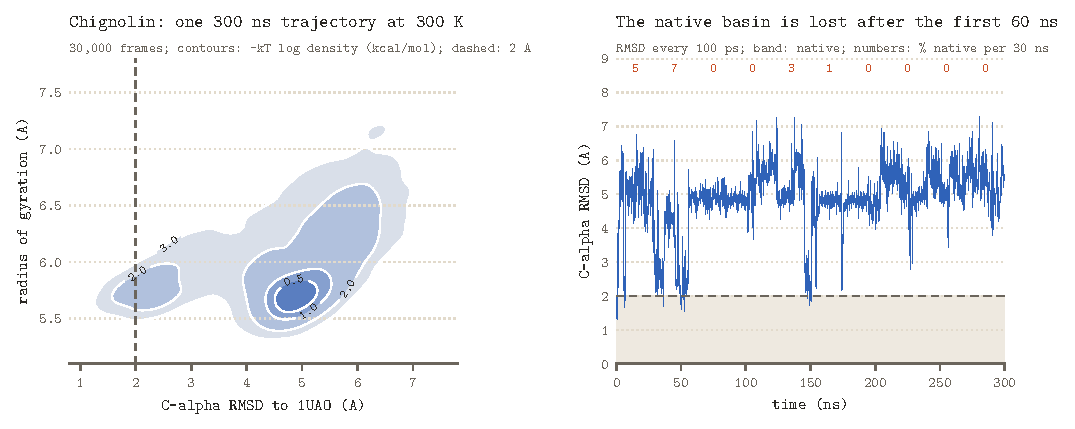
\includegraphics[width=\linewidth]{figures/fig_chignolin_folding_pathology.pdf}
\caption{Chignolin (PDB 1UAO), one 1.0\,$\mu$s trajectory at 300\,K, Amber14/OBC2. Left: $-k_BT\log$ density in (RMSD, $R_g$), kcal/mol relative to the maximum density, from a kernel density estimate on 8{,}000 frames; darker is more populated; dashed: native threshold 2\,\AA; insets: 3D conformations of the native $\beta$-hairpin (1UAO, cobalt) and kinetically trapped misfolded globule (rust). Right: C$\alpha$ RMSD against time; shaded: native region; numbers give the percentage of native frames in each 100\,ns block.}
\label{fig:chignolin_folding}
\end{figure}

\paragraph{Chignolin: Kinetic trapping versus equilibrium benchmarks.}
The continuous 1.0\,$\mu$s trajectory initiates in the native hairpin and leaves it within 60\,ns (Figure~\ref{fig:chignolin_folding}). Across the full microsecond ($\vchigFrames$ frames), the native state accounts for only $\vchigNative\%$ of frames (ten 100\,ns block fractions: $3.7\%$, $0.6\%$, $0\%$, $0\%$, $1.9\%$, $0.4\%$, $0\%$, $10.6\%$, $3.0\%$, $9.8\%$), reflecting persistent kinetic trapping in a non-native misfolded globule. If this non-ergodic fraction represented equilibrium, omitting the native state would shift free energy by only $\vchigBias$\,kcal/mol.

However, converged $100\,\mu$s Anton MD simulations \citep{lindorff2011fastfolding}, open-access multi-microsecond folding ensembles \citep{chignolin_simulations_figshare}, and replica-exchange experiments \citep{honda2008cln025} establish that the true equilibrium native population of chignolin at 300\,K is $\vchigLitNative\%$. Under true thermodynamic equilibrium, omitting the folded hairpin incurs a systematic error of $\vchigLitBias$\,kcal/mol, exceeding the common 0.3\,kcal/mol chemical accuracy standard. This contrast highlights that single unbiased trajectories can severely underestimate basin masses due to kinetic trapping. While the exact numerical equilibrium folded populations ($\vchigLitNative\%$ for chignolin, $\vtrpLitNative\%$ for Trp-cage) are interpreted under Amber14SB/OBC2 and experimental/Anton baselines, and alternative force fields or explicit solvent models may yield shifted equilibrium fractions, the underlying thermodynamic relation $\Delta F = -\beta^{-1}\log(1-\alpha)$ and the inability of self-normalized forward metrics to detect unvisited basins are general physical and mathematical invariants.

\begin{figure}[t]
\centering
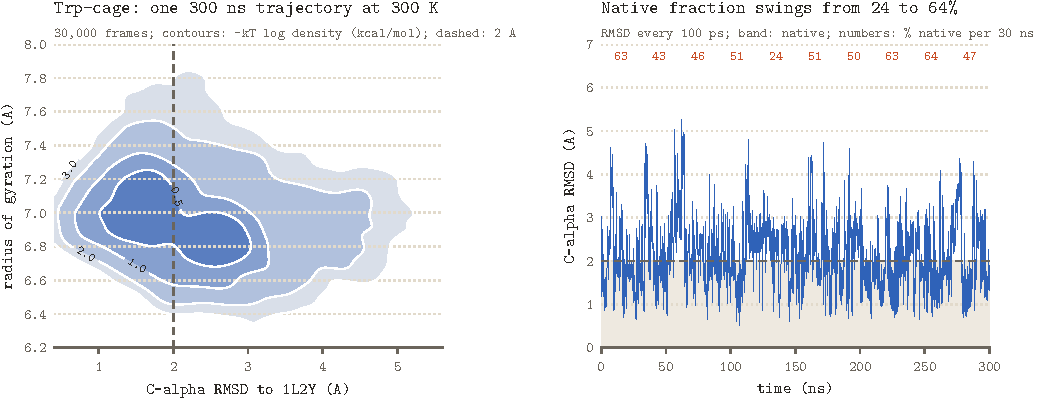
\includegraphics[width=\linewidth]{figures/fig_trpcage_folding_pathology.pdf}
\caption{Trp-cage TC5b (PDB 1L2Y), one 300\,ns trajectory at 300\,K, Amber14/OBC2. Panels as in Figure~\ref{fig:chignolin_folding}.}
\label{fig:trpcage_folding}
\end{figure}

\begin{figure}[t]
\centering
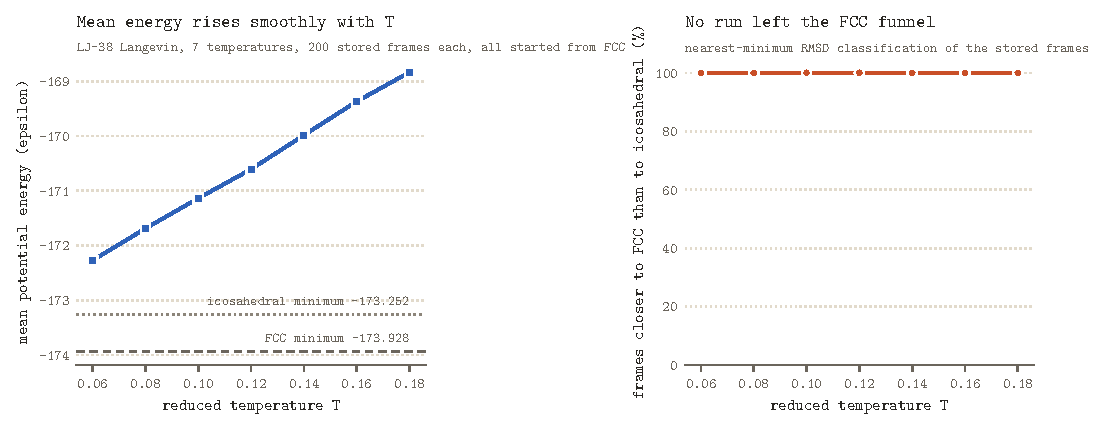
\includegraphics[width=\linewidth]{figures/fig_lj38_entropic_inversion.pdf}
\caption{LJ$_{38}$, Langevin dynamics in reduced units, $\vljNT$ temperatures from $\vljTmin$ to $\vljTmax$, every run started from the FCC minimum, 200 stored frames per temperature. Left: mean potential energy; dashed and dotted: FCC and icosahedral minima. Right: share of stored frames whose RMSD is lower to the FCC minimum than to the icosahedral minimum; insets: 3D structures of the FCC truncated octahedron ($O_h$, global minimum, cobalt) and icosahedral minimum ($C_{5v}$, local minimum, rust).}
\label{fig:lj38_inversion}
\end{figure}

\paragraph{Trp-cage: Macroscopic tertiary packing.}
Trp-cage fluctuates between the native fold and partially unfolded intermediates throughout the 300\,ns run (Figure~\ref{fig:trpcage_folding}; minimum RMSD $\vtrpMinRMSD$\,\AA). The native basin represents $\vtrpNative\%$ of the trajectory (block interval $\vtrpNativeLo$ to $\vtrpNativeHi\%$), corresponding to a free-energy shift of $\vtrpBias$\,kcal/mol (interval $\vtrpBiasLo$ to $\vtrpBiasHi$\,kcal/mol). Converged NMR and explicit-solvent studies \citep{neidigh2002trpcage,lindorff2011fastfolding} place the equilibrium folded fraction at $\vtrpLitNative\%$ at 300\,K, corresponding to a theoretical bias of $\vtrpLitBias$\,kcal/mol. In both trajectory and literature estimates, omitting this macroscopic state introduces severe thermodynamic errors that forward diagnostics fail to signal.

\paragraph{LJ$_{38}$ and double-funnel blindness.}
The 38-atom Lennard-Jones cluster provides a canonical benchmark for double-funnel landscapes \citep{doye1999lj38,wales1999lj38}. Its potential energy global minimum is a face-centered cubic truncated octahedron (FCC, energy $\vljEfcc$), while a dense manifold of icosahedral structures resides slightly higher in potential energy ($\vljEico$). Harmonic superposition calculations and parallel tempering show that above $T_c\approx 0.12$ (reduced units), the icosahedral funnel dominates the equilibrium ensemble, holding $> \vljLitIco\%$ of the Boltzmann mass \citep{doye1999lj38}. 

We performed unbiased Langevin sweeps across $\vljNT$ temperatures from $\vljTmin$ to $\vljTmax$, initializing all trajectories in the FCC minimum. As shown in Figure~\ref{fig:lj38_inversion}, $\vljPfccMin\%$ of stored frames remain classified as FCC across all temperatures. Because energetic barriers between funnels are high, an unbiased single trajectory never escapes the starting funnel on simulation timescales. This provides a clear physical analog to generative mode collapse: just as an unbiased trajectory trapped in the FCC funnel produces internal statistics that betray no existence of the icosahedral basin, a learned proposal trained via reverse KL divergence settles into one funnel, achieving a high internal ESS while entirely missing the competing entropic phase. Accurately resolving both funnels requires enhanced-sampling techniques like parallel tempering, highlighting the necessity of independent reference checks.